\section*{Physique (13 points)}
\section*{Exercice 1 ( 2,5 points)~: Âge approximatif de la Terre}
\section*{La datation par la méthode Uranium-Plomb est une technique ancienne, qui permet la détermination de l'âge approximatif de la Terre.}
Le noyau d'uranium ${ }_{92}^{238} \mathrm{U}$, naturellement radioactif, se transforme en un noyau de plomb ${ }_{\mathrm{Z}}^{\mathrm{A}} \mathrm{Pb}$ stable, après une série de désintégrations successives, parmi lesquelles la désintégration en noyau de thorium ${ }_{90}^{234} \mathrm{Th}$ et la désintégration en noyau de protactinium ${ }_{91}^{234} \mathrm{~Pa}$.

\begin{enumerate}
  \item Recopier sur votre copie le numéro de la question et écrire la lettre correspondante à la proposition vraie parmi~:
\end{enumerate}

\begin{center}
\begin{tabular}{|l|l|}
\hline
a & Le noyau ${ }_{92}^{238} \mathrm{U}$ se désintègre spontanément suivant l'équation ${ }_{92}^{238} \mathrm{U} \longrightarrow{ }_{2}^{4} \mathrm{He}+{ }_{90}^{234} \mathrm{Th}$ \\
\hline
b & Le noyau ${ }_{90}^{234} \mathrm{Th}$ se désintègre spontanément suivant l'équation ${ }_{90}^{234} \mathrm{Th} \longrightarrow{ }_{+1}^{0} \mathrm{e}+{ }_{91}^{234} \mathrm{~Pa}$ \\
\hline
c & La désintégration selon l'équation ${ }_{92}^{238} \mathrm{U} \longrightarrow \longrightarrow{ }_{2}^{4} \mathrm{He}+{ }_{90}^{234} \mathrm{Th}$ est de type $\beta^{-}$ \\
\hline
d & La désintégration selon l'équation ${ }_{90}^{234} \mathrm{Th} \longrightarrow{ }_{90}^{0} \mathrm{e}+{ }_{91}^{234} \mathrm{~Pa}$ est de type $\beta^{+}$ \\
\hline
\end{tabular}
\end{center}

\begin{enumerate}
  \setcounter{enumi}{1}
  \item L'équation ${ }_{92}^{238} \mathrm{U} \longrightarrow{ }_{Z}^{A} \mathrm{~Pb}+6{ }_{-1}^{0} \mathrm{e}+8{ }_{2}^{4} \mathrm{He}$ résume la série de désintégrations successives du noyau ${ }_{92}^{238} \mathrm{U}$ jusqu'au noyau ${ }_{Z}^{A} \mathrm{~Pb}$.
2.1. En appliquant les lois de conservation, trouver les valeurs de A et Z.
2.2. On considère que l'âge de chaque roche minérale ancienne est celui de la Terre qu'on note $\mathrm{t}_{\mathrm{T}}$.
La figure ci-contre représente la courbe de décroissance radioactive des noyaux d'uranium 238 dans un échantillon de roche minérale ancienne contenant $\mathrm{N}_{\mathrm{U}}(0)$ noyaux d'uranium à l'instant $\mathrm{t}_{0}=0$.
\includegraphics[width=\textwidth]{2025_05_10_1877869eca03ab8ede95g-3}
\end{enumerate}

Pour les questions suivantes, recopier sur votre copie le numéro de la question et écrire la lettre correspondante à la proposition vraie parmi~:
2.2.1. La valeur de $\mathrm{N}_{\mathrm{U}}(0)$ est~:

\begin{center}
\begin{tabular}{|c|c|c|c|c|c|c|}
\hline
$\mathbf{a}$ & $2,5.10^{12}$ & $\mathbf{b}$ & $4.10^{12}$ & $\mathbf{c}$ & $4,5.10^{12}$ & $\mathbf{d}$ \\
\hline
\end{tabular}
\end{center}

2.2.2. La demi-vie $t_{1 / 2}$ de l'uranium 238 est~:

\begin{center}
\begin{tabular}{|c|c|c|c|c|c|c|}
\hline
$\mathbf{a}$ & $1,5.10^{9}$ ans & b & $2,25.10^{9}$ ans & c & $4,5.10^{9}$ ans & d \\
\hline
\end{tabular}
\end{center}

2.2.3. La mesure du nombre de noyaux de plomb, dans la roche minérale ancienne, à la date $t_{\mathrm{T}}$, a donné la valeur $\mathrm{N}_{\mathrm{Pb}}\left(\mathrm{t}_{\mathrm{T}}\right)=2,5.10^{12}$.
L'âge approximatif $t_{T}$ de la Terre est~:

\begin{center}
\begin{tabular}{|l|l|l|l|l|l|l|l|}
\hline
$\mathbf{a}$ & $4,5.10^{9}$ ans & b & $2,25.10^{9}$ ans & c & $4,5.10^{10}$ ans & d & $2,25.10^{10}$ ans \\
\hline
\end{tabular}
\end{center}

\section*{Exercice 2 (5 points)~: Dipôle RL-Oscillations électriques libres dans un circuit RLC série}
La bobine, le condensateur et le conducteur ohmique sont des composants
essentiels qu'on trouve dans un ensemble de circuits électriques. Le rôle joué
par ces circuits électriques dépend de la nature de ces composants et des
valeurs des grandeurs qui les caractérisent.

Cet exercice vise à déterminer le rôle joué par une bobine et mettre en évidence
l'influence de la résistance dans un circuit électrique.

\subsection*{Partie 1~: Dipôle RL}
\begin{enumerate}
    \item \mbox{}
          \begin{minipage}[t][][t]{0.62\linewidth}
              Pour étudier l'influence d'une bobine dans un circuit électrique,
              on réalise le montage électrique de la
              Fig.~\ref{fig:2bac_svt_national_2017_rattrapage_phys_ex1_1}, qui
              comporte un générateur idéal de tension, une bobine d'inductance
              $L$ et de résistance $r$, un conducteur ohmique de résistance $R$
              réglable, deux lampes identiques notées $L_{1}$ et $L_{2}$ et un
              interrupteur $\mathrm{K}$.
              
              On règle la résistance du conducteur ohmique sur une valeur
              $R_{0}$ tel que $R_{0}=r$.

              \vspace{2mm}
              Recopier sur votre copie le numéro de la question et écrire la
              lettre correspondante à la proposition vraie parmi~:
          \end{minipage}
          \hfill
          \begin{minipage}[t][][t]{0.34\linewidth}
          \begin{figure}[H]
              \centering
              \begin{circuitikz}
                  \newdimen\d \d=2cm
                  \draw (0,0) coordinate (O)
                      to[vsource,v=$E$] ++(0,2\d)
                      to[cute open switch,l_=$\mathrm{K}$] ++(\d,0)
                      coordinate (A)
                      to[tgeneric,l=$R$,invert] ++(0,-\d)
                      to[lamp,l=$L_{1}$] ++(0,-\d) coordinate (B)
                      to[short] (O);
                \draw (A)
                      to[short] ++(\d,0)
                      to[L,l=$(L{,}r)$] ++(0,-\d)
                      to[lamp,l=$L_{2}$] ++(0,-\d)
                      to[short] (B);
              \end{circuitikz}
              \caption{}
              \label{fig:2bac_svt_national_2017_rattrapage_phys_ex1_1}
          \end{figure}
          \end{minipage}

          \begin{minipage}{\linewidth}
              \begin{table}[H]
              \centering
                  \begin{tabularx}{\textwidth}{|
                      >{\arraybackslash\centering}p{6mm}|L|}
                  \hline
                  $\mathrm{a}$ & Immédiatement après la fermeture de
                  l'interrupteur $\mathrm{K}$, les deux lampes brillent en même
                  temps \\
                  \hline
                  $\mathrm{b}$ & Immédiatement après la fermeture de
                  l'interrupteur $\mathrm{K}$, la lampe $L_{1}$ brille et la
                  lampe $L_{2}$ brille avec un retard \\
                  \hline
                  $\mathrm{c}$ & Immédiatement après la fermeture de
                  l'interrupteur $\mathrm{K}$, la lampe $L_{2}$ brille et la
                  lampe $L_{1}$ brille avec un retard \\
                  \hline
                  $\mathrm{d}$ & Immédiatement après la fermeture de
                  l'interrupteur $\mathrm{K}$, la lampe $L_{1}$ brille et la
                  lampe $L_{2}$ ne brille pas \\
                  \hline
                  \end{tabularx}
              \end{table}
          \end{minipage}

    \item \mbox{}
          \begin{minipage}[t][][t]{0.56\linewidth}
              L'étiquette d'une bobine indique ($L=\qty{60}{\mH}~;
              r=\qty{4}{\ohm}$). Pour vérifier ces deux valeurs, on réalise le
              montage de la
              Fig.~\ref{fig:2bac_svt_national_2017_rattrapage_phys_ex1_2} et on
              règle la résistance du conducteur ohmique sur la valeur
              $R=\qty{8}{\ohm}$.
              
              À l'instant $t_{0}=0$, on ferme l'interrupteur $\mathrm{K}$.
              \begin{enumerate}[itemsep=4pt]
                  \item Montrer que, l'équation différentielle vérifiée par
                        l'intensité $i(t)$ du courant électrique qui circule
                        dans le circuit s'écrit~:
                        $\frac{\mathrm{d}i}{\mathrm{d}t}+\frac{R+r}{L}i=
                        \frac{E}{L}$.
                  \item La solution de cette équation différentielle s'écrit~:
                        $i(t)=A\left(1-e^{-\frac{t}{\tau}}\right)$. Déterminer
                        les expressions des constantes $A$ et $\tau$ en fonction
                        des paramètres du circuit.

                  \item Un système d'acquisition, adéquat, permet de suivre
                        l'évolution au cours du temps des tensions $u_{AB}(t)$
                        et $u_{AM}(t)$. Les courbes~(1) et~(2) traduisant les
                        variations de ces tensions sont représentées sur la
                        Fig.~\ref{fig:2bac_svt_national_2017_rattrapage_phys_ex1_3}.
                        \begin{enumerate}[itemsep=4pt]
                            \item Montrer que la courbe~(2) correspond à la
                                  tension $u_{AB}(t)$.
                            \item Déterminer graphiquement les valeurs de $E$ et
                                  $u_{AB,\max}$.
                            \item Montrer que l'expression de $r$ s'écrit~: \\
                                  $r=R\left(\frac{E}{u_{AB,\max }}-1\right)$.
                                  Vérifier que $r=\qty{4}{\ohm}$.
                            \item Déterminer graphiquement la valeur de la
                                  constante de temps $\tau$, du dipôle RL.
                            \item Vérifier la valeur de l'inductance $L$
                                  indiquée sur l'étiquette.
                        \end{enumerate}
              \end{enumerate}
          \end{minipage}
          \hfill
          \begin{minipage}[t][][t]{0.42\linewidth}
              \begin{figure}[H]
                  \centering
                  \begin{circuitikz}
                      \newdimen\d \d=4cm
                      \draw (0,0)
                          to[vsource,v=$E$] ++(0,\d)
                          to[cute open switch,l=$\mathrm{K}$,-*] ++(0.8\d,0)
                          node[right] {$\mathrm{A}$}
                          to[R,l=$R$,i>_=$i$,-*] ++(0,-0.5\d)
                          node[right] {$\mathrm{B}$}
                          to[L,l={$(L,r)$},-*,name=C] ++(0,-0.5\d)
                          node[right] {$\mathrm{M}$}
                          to[short] (0,0);
                  \end{circuitikz}
                  \caption{}
                  \label{fig:2bac_svt_national_2017_rattrapage_phys_ex1_2}
              \end{figure}
              \begin{figure}[H]
                  \centering
                  \flushright
                  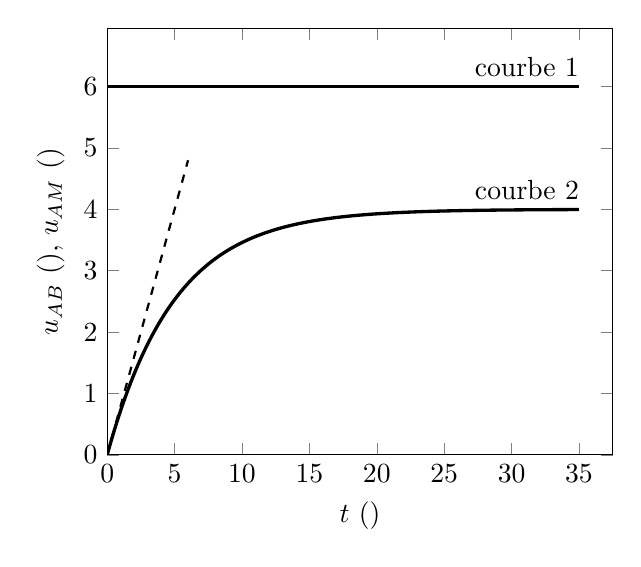
\begin{tikzpicture}
                      \def\A{4}
                      \def\ta{5}
                      \begin{axis}[
                              samples=200,
                              xmin=0,xmax=37.5,
                              ymin=0,ymax=6.95,
                              width=8cm,height=7cm,
                              xtick distance=5,
                              ytick distance=1,
                              xlabel=$t~(\unit{\ms})$,
                              ylabel=
                              {$u_{AB}~(\unit{\volt})$, $u_{AM}~(\unit{\volt})$},
                          ]
                          \addplot[
                                  domain=0:35,
                                  very thick,black
                                  ] {\A*(1-exp(-\x/\ta))}
                                  coordinate[pos=1.02](C1);
                          \addplot[
                                  domain=0:6,
                                  black,thick,dashed
                              ] {\A*\x/\ta)};
                          \addplot[
                                  domain=0:35,
                                  very thick,black
                              ] {6} coordinate[pos=1.02](C2);
                      \end{axis}
                      \node[above left] at (C1) {courbe~2};
                      \node[above left] at (C2) {courbe~1};
                  \end{tikzpicture}
                  \caption{}
                  \label{fig:2bac_svt_national_2017_rattrapage_phys_ex1_3}
              \end{figure}
          \end{minipage}
\end{enumerate}


\section*{Partie 2~: Oscillations électriques libres dans un circuit RLC série}
On monte, en série, la bobine et le conducteur ohmique précédents avec un condensateur de capacité C préalablement chargé. Les courbes (1), (2) et (3) représentent les variations de la tension $\mathrm{u}_{\mathrm{C}}(\mathrm{t})$ entre les bornes du condensateur pour différentes valeurs de la résistance du conducteur ohmique.
\includegraphics[width=\textwidth]{2025_05_10_1877869eca03ab8ede95g-5(2)}

\begin{enumerate}
  \item Recopier le tableau suivant sur votre copie et le compléter en associant le numéro de la courbe à la valeur de la résistance R qui lui correspond.
\end{enumerate}

\begin{center}
\begin{tabular}{|c|c|c|c|}
\cline { 2 - 4 }
\multicolumn{1}{c|}{} & $\mathrm{R}=10 \Omega$ & $\mathrm{R}=20 \Omega$ & $\mathrm{R}=123 \Omega$ \\
\hline
numéro de la courbe & $\ldots \ldots$ & $\ldots \ldots$ & $\ldots$. \\
\hline
\end{tabular}
\end{center}

\begin{enumerate}
  \setcounter{enumi}{1}
  \item On considère la courbe (1)~:
2.1. Déterminer la valeur de la pseudo période T des oscillations électriques.
2.2. En supposant que la pseudo période $T$ est égale à la période propre $T_{0}$ des oscillations libres de l'oscillateur (LC), vérifier que la valeur de la capacité est $C=15 \mu F$ (On prendra $\pi^{2}=10$ ).
\end{enumerate}


\input{physique_ex3.tex}


\section*{Exercice 3 (5,5 points)~: Étude dynamique et étude énergétique du mouvement d'un solide}
Les mouvements des solides sont liés aux actions mécaniques qu'ils subissent et qu'on modélise par des forces.
Le but de cet exercice est l'étude du mouvement d'un solide ( S ) de centre d'inertie G et de masse $m$ dans deux situations différentes.

\section*{1. Etude du mouvement d'un solide sur un plan incliné}
On lance, à l'instant $\mathrm{t}_{0}=0$, un solide $(\mathrm{S})$ de la position O avec une vitesse initiale $\overrightarrow{\mathrm{v}}_{0}=\mathrm{v}_{0} . \overrightarrow{\mathrm{i}}$. Le solide glisse selon la ligne de plus grande pente d'un plan incliné d'un angle $\alpha$ par rapport à l'horizontale. On étudie le mouvement de G, dans le repère ( $\mathrm{O}, \overrightarrow{\mathrm{i}}, \overrightarrow{\mathrm{j}}$ ) lié à la Terre supposé galiléen (figure1).
\includegraphics[width=\textwidth]{2025_05_10_1877869eca03ab8ede95g-6}

Figure 1 L'abscisse de $G$ à $t_{0}=0$ est $x_{G}=x_{0}=0$.
Données~: $\mathrm{m}=0,2 \mathrm{~kg}~; \mathrm{g}=10 \mathrm{~m} . \mathrm{s}^{-2}~; \mathrm{v}_{0}=2 \mathrm{~m} . \mathrm{s}^{-1}~; \alpha=11^{\circ}$
1.1. On suppose les frottements négligeables.
1.1.1. En appliquant la deuxième loi de Newton, exprimer l'accélération $a_{1}$ du mouvement de $G$ en fonction de $g$ et $\alpha$.
Déduire la nature du mouvement de G .
1.1.2. Écrire l' expression numérique de l'équation horaire du mouvement de G.
1.2. La chronophotographie du mouvement de (S) à l'aide d'un système d'acquisition convenable a permis d'obtenir la courbe de la figure (2) qui donne les variations de la vitesse $\mathrm{v}_{\mathrm{G}}$ de G en fonction du temps.
\includegraphics[width=\textwidth]{2025_05_10_1877869eca03ab8ede95g-6(1)}
1.2.1. Déterminer graphiquement la valeur expérimentale de l'accélération $a_{2}$ du mouvement de $G$.
1.2.2. Montrer que le mouvement de G se fait avec frottement.
1.2.3. Les frottements auxquels est soumis le solide (S) sont équivalents à une force $\vec{f}$ constante colinéaire à la vitesse $\vec{v}$ et de sens contraire. Déterminer l'intensité de la force $\vec{f}$.

\subsection{Étude du mouvement d'un oscillateur \{solide (S), ressort\}}
\begin{minipage}{0.64\linewidth}
Le solide $(S)$ précédent de masse $m=\qty{0,2}{\kg}$ est fixé à un ressort
horizontal à spires non jointives, de masse négligeable et de raideur $K$.

À l'équilibre, le centre d'inertie $G$ coïncide avec l'origine du repère
($O,\ex$) lié à la terre considéré comme galiléen
(figure~\ref{fig:solide_ressort}). On écarte le solide $(S)$ de sa position
d'équilibre d'une distance $X_{m}=\qty{2}{\cm}$ et on le libère sans vitesse
initiale à l'instant $t_{0}=0$. Le solide $(S)$ est animé d'un mouvement de
translation rectiligne sinusoïdal.

On choisit l'état où le ressort n'est pas déformé comme référence de l'énergie
potentielle élastique $E_{pe}$ et le plan horizontal contenant $G$ comme état de
référence de l'énergie potentielle de pesanteur $E_{pp}$.

La figure~(\ref{fig:Ec_et_Epe_de_t}) représente les variations de l'énergie
potentielle élastique $E_{pe}$ et de l'énergie cinétique $E_{c}$ en fonction du
temps pour l'oscillateur étudié.
\end{minipage}
\hfill
\begin{minipage}{0.35\linewidth}
\begin{figure}[H]
    \centering
    \begin{tikzpicture}
    \node[inner sep=0pt,minimum width=4.5cm,minimum height=3mm,
        top color=black!70] (sol) {};
    % Axe xx'
    \coordinate (O) at ($(sol.south west)!.8!(sol.south east)$);
    \draw[-Latex] (sol.south west)
        node[below right,inner xsep=0pt] {$x^{\prime}$} -- (O)
        node[below=0.4mm] {$O$} -- (sol.south east) -- ++(0.7,0)
        node[below left,inner xsep=0pt,inner ysep=2mm] {$x$};
    % Fixed
    \node[inner sep=0pt,draw,minimum width=3mm,minimum height=7mm,
        anchor=south,pattern=north west lines,
        thick] (fix) at ([xshift=3mm,yshift=0.4pt]sol.north west) {};
    % Solide (S)
    \node[inner sep=0pt,draw,minimum width=7mm,minimum height=7mm,
        anchor=south,rounded corners=2pt,thick,label=$\mathrm{(S)}$,
        fill=lightgray] (S) at
        ([yshift=0.4pt]O |- sol.north) {};
        %([xshift=-6mm,yshift=0.4pt]sol.north east) {};
    \node[inner sep=1pt,circle,fill,
        label={[right=-0.8mm,font=\scriptsize]:$G$}] (G) at (S.center) {};
    \draw[{Rectangle[length=1pt,width=4pt]}-{Stealth[length=5pt]},
        thick] (O) -- ++(0.8,0)
        node[below left,inner xsep=0pt] {$\ex$};
    % Ressort
    \draw[decoration={
          coil,
          aspect=0.3,
          segment length=2.0mm,
          amplitude=2.4mm,
          pre length=1mm,
          post length=1mm},
          decorate,thick,black] (fix.east) -- (S.west);
\end{tikzpicture}

    \caption{}
    \label{fig:solide_ressort}
\end{figure}
\begin{figure}[H]
    \centering
    \begin{tikzpicture}
        \def\Xm{0.02}
        \def\T{1}
        \def\K{8}
        \pgfmathpi\let\pi=\pgfmathresult
        \begin{axis}[
                xmin=0,xmax=1.69,
                ymin=0,ymax=2.19,
                width=8cm,height=6.5cm,
                trig format plots=rad,
                xtick distance=0.25, ytick distance=0.4,
                xticklabels={,,{0,25}}, yticklabels={,,{0,4}},
                xlabel=$t~(\unit{\second})$,
                ylabel=$E_{c}~(\unit{\mJ})~;~E_{pe}~(\unit{\mJ})$,
            ]
            \addplot[domain=0~:1.5,samples=200,thick,blue]
                {0.5*\K*\Xm*\Xm*cos(2*pi/\T*x)*cos(2*pi/\T*x)*1e3}
                coordinate[pos=0.68] (c1)~;
            \addplot[domain=0~:1.5,samples=200,very thick,red]
                {0.5*\K*\Xm*\Xm*sin(2*pi/\T*x)*sin(2*pi/\T*x)*1e3}
                coordinate[pos=0.18] (c2)~;
        \end{axis}
        \draw[<-,shorten <=1pt] (c1) -- ++(50~:1) node[right,draw] {courbe~1}~;
        \draw[<-,shorten <=1pt] (c2) -- ++(50~:1) node[right,draw] {courbe~2}~;
    \end{tikzpicture}
    \caption{}
    \label{fig:Ec_et_Epe_de_t}
\end{figure}
\end{minipage}
\begin{enumerate}
    \item Montrer, que la courbe~(2) correspond à l'énergie cinétique $E_{c}$ du
          système oscillant.
    \item Déterminer graphiquement, la valeur de l'énergie potentielle élastique
          maximale $E_{pe,\max}$.
    \item En déduire la valeur de la raideur $K$.
    \item Déterminer la valeur de la vitesse $v_{G}$ du centre d'inertie $G$
          lorsque $E_{c}=E_{pe}$.
\end{enumerate}

